\documentclass[tikz,border=2pt]{standalone}
\usepackage{amsmath}
\usepackage{pgfplots}
\pgfplotsset{compat=1.18}
\usetikzlibrary{arrows.meta}

\begin{document}
% f(x)=x^2 on [0,2] and its inverse sqrt(y): the graphs are mirror images in y=x,
% so the tangent at (x0,f(x0)) with slope f'(x0) reflects to the tangent at
% (f(x0),x0) with slope 1/f'(x0). Here x0=1.2, f'(x0)=2.4.
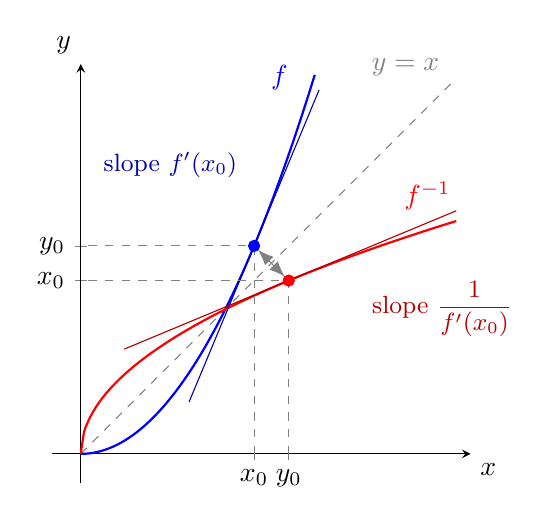
\begin{tikzpicture}
	\begin{axis}[
		axis lines=middle,
		axis equal image,
		xmin=-0.2, xmax=2.7,
		ymin=-0.2, ymax=2.7,
		xtick={1.2,1.44}, xticklabels={$x_0$,$y_0$},
		ytick={1.2,1.44}, yticklabels={$x_0$,$y_0$},
		xlabel={$x$}, ylabel={$y$},
		xlabel style={below right}, ylabel style={above left},
		samples=120, smooth, clip=false,
		width=8cm
		]
		% the mirror line
		\addplot[gray, dashed, domain=0:2.6] {x};
		\node[gray, anchor=south east] at (axis cs:2.55,2.55) {$y=x$};
		% f and its inverse
		\addplot[thick, blue, domain=0:1.62] {x^2};
		\node[blue, anchor=south east] at (axis cs:1.5,2.45) {$f$};
		\addplot[thick, red, domain=0:2.6] {sqrt(x)};
		\node[red, anchor=south] at (axis cs:2.4,1.62) {$f^{-1}$};
		% tangents: slope 2.4 at (1.2,1.44), slope 1/2.4 at (1.44,1.2)
		\addplot[blue!70!black, thin, domain=0.75:1.65] {2.4*(x-1.2)+1.44};
		\addplot[red!70!black, thin, domain=0.3:2.6] {(x-1.44)/2.4+1.2};
		% the two mirror points and their coordinate lines
		\draw[dashed, gray] (axis cs:1.2,0) -- (axis cs:1.2,1.44) -- (axis cs:0,1.44);
		\draw[dashed, gray] (axis cs:1.44,0) -- (axis cs:1.44,1.2) -- (axis cs:0,1.2);
		\draw[gray, {Latex[length=2mm]}-{Latex[length=2mm]}, shorten >=2pt, shorten <=2pt] (axis cs:1.2,1.44) -- (axis cs:1.44,1.2);
		\addplot[only marks, mark=*, blue] coordinates {(1.2,1.44)};
		\addplot[only marks, mark=*, red] coordinates {(1.44,1.2)};
		\node[blue!70!black, anchor=east, font=\small] at (axis cs:1.15,2.0) {slope $f'(x_0)$};
		\node[red!70!black, anchor=west, font=\small] at (axis cs:1.95,1.0) {slope $\dfrac{1}{f'(x_0)}$};
	\end{axis}
\end{tikzpicture}
\end{document}
